%\documentclass[a4paper,11pt]{article}
\documentclass{article}
%%%%%%%%%%%%%%%%%%%%%%%%%%%%%%%%%%%%%%%%%%%%%%%%%%%%%%%%%%%%%%%%%%%%%%%%%%%%%%%%%%%%%%%%%%%%%%%%%%%%%%%%%%%%%%%%%%%%%%%%%%%%
\usepackage{graphics,graphicx}
\usepackage{amsmath,amssymb,graphics,graphicx}
\usepackage[ansinew]{inputenc}
\usepackage[usenames,dvipsnames]{color}

\graphicspath{{Images/}}
\usepackage{natbib}

\bibpunct{(}{)}{;}{a}{,}{,}

\textheight 24cm \textwidth 17cm \topmargin-2cm
%% \evensidemargin   -0.25cm
\oddsidemargin-0.2cm
%\pagestyle{empty}
\renewcommand{\baselinestretch}{1}

\begin{document}

\title{Pr\'actica 1: FIFA Players Classification}

\author{{Daniel Carmona Pedrajas}}

\date{}
\maketitle

%\title{}

%\address{}

		
    \section{Arquitectura Borja}
			Probaremos una arquitectura de complejidad media para buscar el overfitting y aplicaremos t\'ecnicas de regularizaci\'on para reducir la varianza. 
			\begin{itemize}
			    \item Capa densa de 256 con Batch Normalization y Dropout = 0
                \item Capa densa de 124 con BN y Dropout = 0
                \item Capa densa de 64 con BN y Dropout = 0
                \item Capa densa de 32 con BN y Dropout = 0
			\end{itemize}
		\subsection{Experimento 1: Primera configuraci\'on}
        \label{s-a6-e1}
            Como se puede observar en la figura \ref{tab:tr-a6-e1}, tenemos un overfitting bastante grande y debemos aplicar t\'ecnicas de regularizaci\'on para mejorar la generalizaci\'on de la red. 
            \begin{table}[!h]
				\begin{tabular}{|c|c|c|c|c|c|c|c|c|}
					\textbf{Epochs}&\textbf{L.R}&\textbf{Batch size}&\textbf{Activation}&\textbf{Loss}&\textbf{Optimizer}&\textbf{Regularization}&\textbf{Dropout}   \\ \hline
					400 & 0.001 & 64 & ReLU & C.C. & ADAM & No & 0 
				\end{tabular}
				\caption{Hiperpar\'ametros para el Experimento 1 de la Arquitectura 6}
				\label{tab:hip-a6-e1}
			\end{table}
   
            \begin{table}[!h]
				\begin{center}
					\begin{tabular}{ c | c | c | c | c | c |}
						\ & \textbf{Train accuracy (\%)} & \textbf{Validation accuracy (\%)} & \textbf{Bias (\%)} & \textbf{Variance (\%)} & \textbf{Training time (s)} \\ \hline
						\textbf{Mean} & 98.7 & 70.47 & -3.7  & 28.23 & 817   \\ \hline
						\textbf{Std} &  0.83 & 0.28 &  0.83 & 0.86 & 8.4  \\ \hline
					\end{tabular}
					\caption{Resultados del Experimento 1 de la Arquitectura 6}
					\label{tab:res-a2-e5}
				\end{center}
			\end{table}
            
            \begin{figure}[!h]
				\begin{center}
					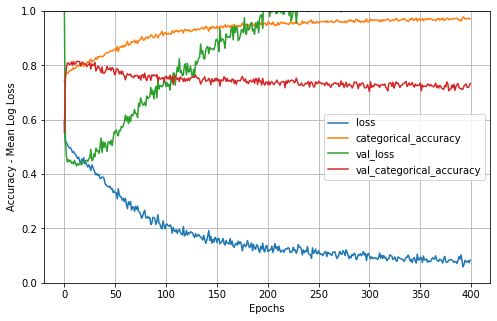
\includegraphics[scale=0.5]{tr-a6-e1.png}		
					\caption{Entrenamiento durante el Experimento 1 de la Arquitectura 6}	
					\label{tab:tr-a6-e1}
				\end{center}
			\end{figure}
   
        \subsection{Experimento 2: A\~{n}adimos Dropout 0.2}
        \label{s-a6-e2}
            Se a\~{n}ade un Dropout de 0.2 para reducir la varianza y mejorar la generalizaci\'on. La configuraci\'on es la siguiente: 
   
            \begin{table}[!h]
				\begin{tabular}{|c|c|c|c|c|c|c|c|c|}
					\textbf{Epochs}&\textbf{L.R}&\textbf{Batch size}&\textbf{Activation}&\textbf{Loss}&\textbf{Optimizer}&\textbf{Regularization}&\textbf{Dropout}   \\ \hline
					400 & 0.001 & 64 & ReLU & C.C. & ADAM & No & 0.2 
				\end{tabular}
				\caption{Hiperpar\'ametros para el Experimento 1 de la Arquitectura 6}
				\label{tab:hip-a6-e2}
			\end{table}
   
            Los resultados obtenidos son los siguientes: 
            \begin{table}[!h]
				\begin{center}
					\begin{tabular}{ c | c | c | c | c | c |}
						\ & \textbf{Train accuracy (\%)} & \textbf{Validation accuracy (\%)} & \textbf{Bias (\%)} & \textbf{Variance (\%)} & \textbf{Training time (s)} \\ \hline
						\textbf{Mean} & 88.28  & 76.67 & 6.72 & 11.61 & 743  \\ \hline
						\textbf{Std} & 1.15  & 0.79 & 1.15 & 1.89 & 8.9  \\ \hline
					\end{tabular}
					\caption{Resultados del Experimento 2 de la Arquitectura 6}
					\label{tab:res-a2-e5}
				\end{center}
			\end{table}
            \begin{figure}[!h]
				\begin{center}
					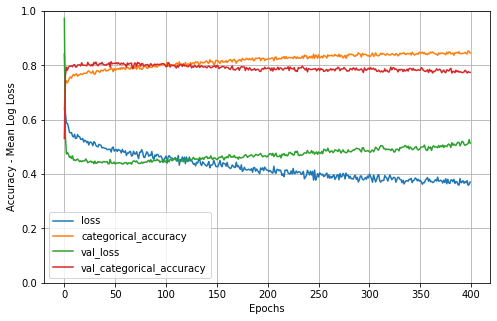
\includegraphics[scale=0.5]{tr-a6-e2.png}		
					\caption{Entrenamiento durante el Experimento 2 de la Arquitectura 6}	
					\label{tab:tr-a6-e2}
				\end{center}
			\end{figure}
            Se consigue una reducci\'on de la varianza a cambio de un empeoramiento del Bias. 
        
        \subsection{Experimento 3: Regularizac\'on L1, L2 y L1-L2 }
        Seguimos buscando la reducci\'on de la varianza. Para ello probaremos los regularizadores L1, L2 y L1-L2. 


      
        \begin{table}[!h]
				\begin{tabular}{|c|c|c|c|c|c|c|c|c|}
					\textbf{Epochs}&\textbf{L.R}&\textbf{Batch size}&\textbf{Activation}&\textbf{Loss}&\textbf{Optimizer}&\textbf{Regularization}&\textbf{Dropout}   \\ \hline
					400 & 0.001 & 64 & ReLU & C.C. & ADAM & ? & 0.2 
				\end{tabular}
				\caption{Hiperpar\'ametros para el Experimento 3 de la Arquitectura 6}
				\label{tab:hip-a6-e2}
			\end{table}

    
   
   \begin{table}[!h]
				\begin{center}
					\begin{tabular}{ c | c | c | c | c | c |}
						\ & \textbf{Train accuracy (\%)} & \textbf{Validation accuracy (\%)} & \textbf{Bias (\%)} & \textbf{Variance (\%)} & \textbf{Training time (s)} \\ \hline
						\textbf{L1 0.1} &63.6   &68.98  & 31.4  & -5.38 &  765 \\ \hline
						\textbf{L2 0.1} & 73.06   & 76.86 &  21.94 & -3.8 &864   \\ \hline
                        \textbf{L1-L2 0.1} &  63.7  &72.02 &  31.3 & -8.32 &804   \\ \hline
					\end{tabular}
					\caption{Resultados del Experimento 3 de la Arquitectura 6}
					\label{tab:res-a2-e5}
				\end{center}
			\end{table}
   
   \begin{figure}[!h]
				\begin{center}
					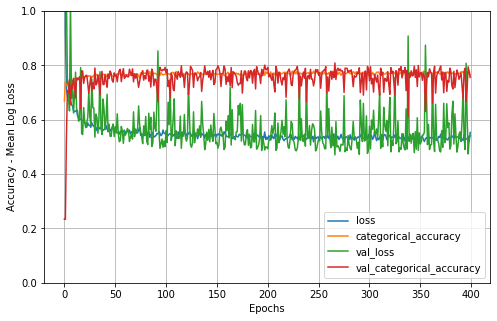
\includegraphics[scale=0.5]{tr-a6-e3.1.png}		
					\caption{Entrenamiento durante el Experimento 3 (L2) de la Arquitectura 6}	
					\label{tab:tr-a6-e2}
				\end{center}
			\end{figure}
    Como se puede observar la regularizac\'on L1 ha mejorado drasticamente la varianza y se ha conseguido una configuraci\'on que generaliza mejor. Sin embargo se ha aumentado demasiado el Bias, es por ello que en los siguientes experimentos habr\'a que intentar reducir el Bias. 
    
           La regularizac\'on L2 tambien ha conseguido reducir considerablemente la varianza, pero tiene la ventaja de que hemos conseguido menor empeoramiento que con L1. Se concluuye que en este caso es comveniente usar L2 frente a L1. En los siguientes experimentos habr\'a que intentar reducir el Bias, las soluciones partir\'ian de una reducci\'on del tama\~{n}o del Batch hasta una aumento de epochs. 
           
  La regularizaci\'on L1-L2 tambi\'en mejora dr\'asticamente la varianza, pero empeora en exceso el Bias. 

  Se concluye que el mejor regularizador para nuestra configuraci\'on actual es el L1. 
  
   

   
        \subsection{Experimento 4: Aumentar Epochs}
        En el experimento anterior se ha conseguido una mejora de la generalizaci\'on de la red a cambio de un alto Bias, es por ello que en este experimento se busca la reducci\'on del Bias utilizando m\'as epochs de entrenamiento. 
        
        \begin{table}[!h]
				\begin{tabular}{|c|c|c|c|c|c|c|c|c|}
					\textbf{Epochs}&\textbf{L.R}&\textbf{Batch size}&\textbf{Activation}&\textbf{Loss}&\textbf{Optimizer}&\textbf{Regularization}&\textbf{Dropout}   \\ \hline
					? & 0.001 & 64 & ReLU & C.C. & ADAM & L2 0.1 & 0.2 
				\end{tabular}
				\caption{Hiperpar\'ametros para el Experimento 3 de la Arquitectura 6}
				\label{tab:hip-a6-e2}
			\end{table}

    
   
   \begin{table}[!h]
				\begin{center}
					\begin{tabular}{ c | c | c | c | c | c |}
						 \textbf{epochs} & \textbf{Train accuracy (\%)} & \textbf{Validation accuracy (\%)} & \textbf{Bias (\%)} & \textbf{Variance (\%)} & \textbf{Training time (s)} \\ \hline
						\textbf{400 } & 73.06   & 76.86 &  21.94 & -3.8 &864   \\ \hline
                        \textbf{800 } & 73.52   &77.98 &  21.48 & -4.46  &1585    \\ \hline
                        \textbf{1200} &  72.64  &75.37  &  22.36& -2.73 &1944    \\ \hline
					\end{tabular}
					\caption{Resultados del Experimento 4 de la Arquitectura 6}
					\label{tab:res-a2-e5}
				\end{center}
			\end{table}

Duplicando o triplicando el n\'umero de epochs no se est\'a logrando una mejora significativa de la varianza. Esto puede ser debido a que la red se est\'a quedando atrapada en un m\'inimo local y hay que aplicar más reconfiguraciones para solventar este problema. 
\subsection{Experimento 5: Optimizadores}
Se van a probar los diferentes optimizadores con los hiper par\'ametros por defecto para buscar una mejor aproximaci\'on e intentar salir en el m\'inimo local en que se encuentra la red. 

 \begin{table}[!h]
				\begin{tabular}{|c|c|c|c|c|c|c|c|c|}
					\textbf{Epochs}&\textbf{L.R}&\textbf{Batch size}&\textbf{Activation}&\textbf{Loss}&\textbf{Optimizer}&\textbf{Regularization}&\textbf{Dropout}   \\ \hline
					400 & 0.001 & 64 & ReLU & C.C. & ? & L2 0.1 & 0.2 
				\end{tabular}
				\caption{Hiperpar\'ametros para el Experimento 5 de la Arquitectura 6}
				\label{tab:hip-a6-e2}
			\end{table}

    
   
   \begin{table}[!h]
				\begin{center}
					\begin{tabular}{ c | c | c | c | c | c |}
						 \textbf{Batch Size} & \textbf{Train accuracy (\%)} & \textbf{Validation accuracy (\%)} & \textbf{Bias (\%)} & \textbf{Variance (\%)} & \textbf{Training time (s)} \\ \hline
						\textbf{Adam } & 73.06   & 76.86 &  21.94 & -3.8 &864   \\ \hline
                        \textbf{RMSprop } & 71.39   &79.53  & 23.61  & -8.14  &  865   \\ \hline
                        \textbf{SGD} &  77.42   &  78.35& 17.58 & -0.93 &   683  \\ \hline
					\end{tabular}
					\caption{Resultados del Experimento 5 de la Arquitectura 6}
					\label{tab:res-a2-e5}
				\end{center}
			\end{table}
   
   \begin{figure}[!h]
				\begin{center}
					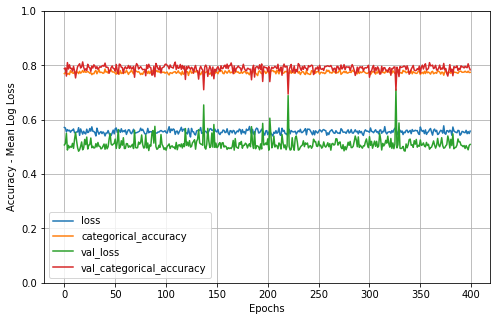
\includegraphics[scale=0.5]{Images/tr-a6-e5(SGD).png}		
					\caption{Entrenamiento durante el Experimento 5 (SGD) de la Arquitectura 6}	
					\label{tab:tr-a6-e2}
				\end{center}
			\end{figure}
   
   Como se puede observar con el optimizador SGD se consigue una liguera mejora en los resultados. Sin embargo, creemos que se puede conseguir mejores resultados ya que el Bias sigue siendo demasiado alto y la curva de aprendizaje es plana, lo que nos puede indicar que seguimos atrapados en un mínimo local. 
   \subsection{Experimento 6: Variando el Batch size}

Se sigue buscando una reducci\'on del Bias, para ello en este experimento se probar\'an diferentes tama\~{n}os de Batch para comprobar si se consigue una mejora. 

    \begin{table}[!h]
				\begin{tabular}{|c|c|c|c|c|c|c|c|c|}
					\textbf{Epochs}&\textbf{L.R}&\textbf{Batch size}&\textbf{Activation}&\textbf{Loss}&\textbf{Optimizer}&\textbf{Regularization}&\textbf{Dropout}   \\ \hline
					400 & 0.001 & ?& ReLU & C.C. & SGD & L2 0.1 & 0.2 
				\end{tabular}
				\caption{Hiperpar\'ametros para el Experimento 6 de la Arquitectura 6}
				\label{tab:hip-a6-e2}
			\end{table}

    
   
   \begin{table}[!h]
				\begin{center}
					\begin{tabular}{ c | c | c | c | c | c |}
						 \textbf{Optimizer} & \textbf{Train accuracy (\%)} & \textbf{Validation accuracy (\%)} & \textbf{Bias (\%)} & \textbf{Variance (\%)} & \textbf{Training time (s)} \\ \hline
	
                        \textbf{64} &  77.42   &  78.35& 17.58 & -0.93 &   683  \\ \hline
                        \textbf{32} &  73.9    & 79.16& 21.1 & -5.26 &   863  \\ \hline
                        \textbf{128} &  81.24  &  79.53& 13.76 &  1.71  &   443   \\ \hline
                        \textbf{256} &  84.74 &  78.47 & 10.26 & 6.27 &   383    \\ \hline
					\end{tabular}
					\caption{Resultados del Experimento 6 de la Arquitectura 6}
					\label{tab:res-a2-e5}
				\end{center}
			\end{table}
   

    \subsection{Experimento 7: Variando el Learning Rate}

     \begin{table}[!h]
				\begin{tabular}{|c|c|c|c|c|c|c|c|c|}
					\textbf{Epochs}&\textbf{L.R}&\textbf{Batch size}&\textbf{Activation}&\textbf{Loss}&\textbf{Optimizer}&\textbf{Regularization}&\textbf{Dropout}   \\ \hline
					400 & ?  & 64 & ReLU & C.C. & SGD & L2 0.1 & 0.2 
				\end{tabular}
				\caption{Hiperpar\'ametros para el Experimento 7 de la Arquitectura 6}
				\label{tab:hip-a6-e2}
			\end{table}

    
   
   \begin{table}[!h]
				\begin{center}
					\begin{tabular}{ c | c | c | c | c | c |}
						 \textbf{Learning Rate} & \textbf{Train accuracy (\%)} & \textbf{Validation accuracy (\%)} & \textbf{Bias (\%)} & \textbf{Variance (\%)} & \textbf{Training time (s)} \\ \hline
	
                        \textbf{0.001} &    &  78.35& 17.58 & -0.93 &   683  \\ \hline
                        \textbf{0.01} &      & 79.16& 21.1 & -5.26 &   863  \\ \hline
                        \textbf{0.1} &   &  78.35& 17.58 & -0.93 &   683  \\ \hline
					\end{tabular}
					\caption{Resultados del Experimento 7 de la Arquitectura 6}
					\label{tab:res-a2-e5}
				\end{center}
			\end{table}
\end{document}
